\documentclass[main]{subfiles}

\begin{document}

At the beginning, the number of \ac{PP} has been chosen to be 

\begin{equation}
    PP = 4
\end{equation}

Because it has been evaluated as a good tradeoff beetween sinewaves maximum 
frequency and amplitude and mechanical robustness.
The $4$ \ac{PP} target is solid enough to be realized using aluminium instead of 
another \ac{PCB} and this has been another key factor for the choice.

The target design is shown in figure \ref{FIG_AL_TARGET}.
Its external diameter is constrained to $50 mm$ because of mounting constraints,
and it is divided into $8$ sectors of $45^\circ$ amplitude.

\begin{figure}
    \centering
    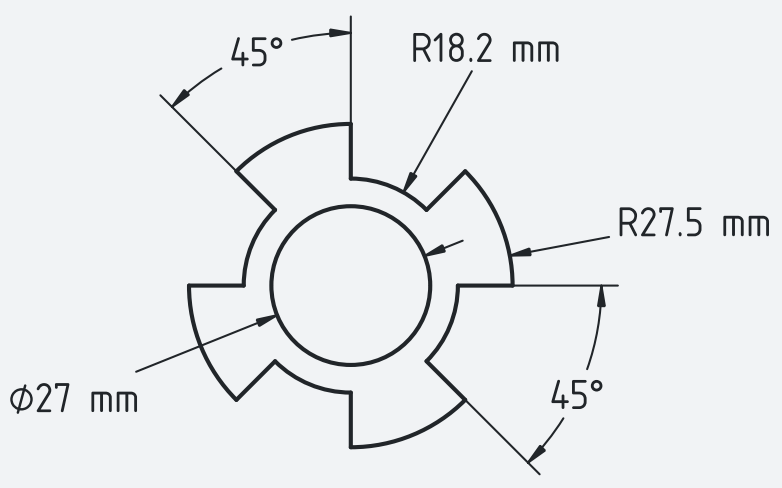
\includegraphics[width=0.7\linewidth]{img/target_meas.png}
    \caption{Aluminuim target}
    \label{FIG_AL_TARGET}
\end{figure}

The encoder hardware has been divided into some hardware blocks, that can be seen 
in figure \ref{FIG_HW_BLOCKS}.

\begin{figure}[h]
    \centering
    
\includegraphics[width=\linewidth]{img/HW_blocks.png}
    \caption{Hardware block scheme}
    \label{FIG_HW_BLOCKS}
\end{figure}

\begin{figure}[h]
    \centering
    
\includegraphics[width=\linewidth]{img/HW_blocks_pwr.png}
    \caption{Hardware block scheme}
    \label{FIG_HW_BLOCKS_PWR}
\end{figure}

There is a power supply which takes the input voltage from $5 V$ to $32 V$, and 
generates the $3.3 V$ supply rail for the whole board (figure \ref{FIG_HW_BLOCKS_PWR}).

The main block is the coil interface (figure \ref{HW_BLOCK_COIL_IF_IC}), which 
is composed of the coil interface \ac{IC} and some passive components around it.
This \ac{IC} needs some capacitors to produce a resonant circuit with the TX coil.
In this way the coil current becomes purely sinusoidal, and its amplitude is maximized.
The \ac{IC} is able to follow the resonance of the circuit, so the exiting frequency
will always be the resonant frequency, and it can be chosen as 

\begin{equation}
    f_{ex} = \frac{1}{2\pi \sqrt{L_{TX}C_{p}}} 
\end{equation}

The other components create some filters to cope with high frequency noise.

\begin{figure}[h]
    \centering
    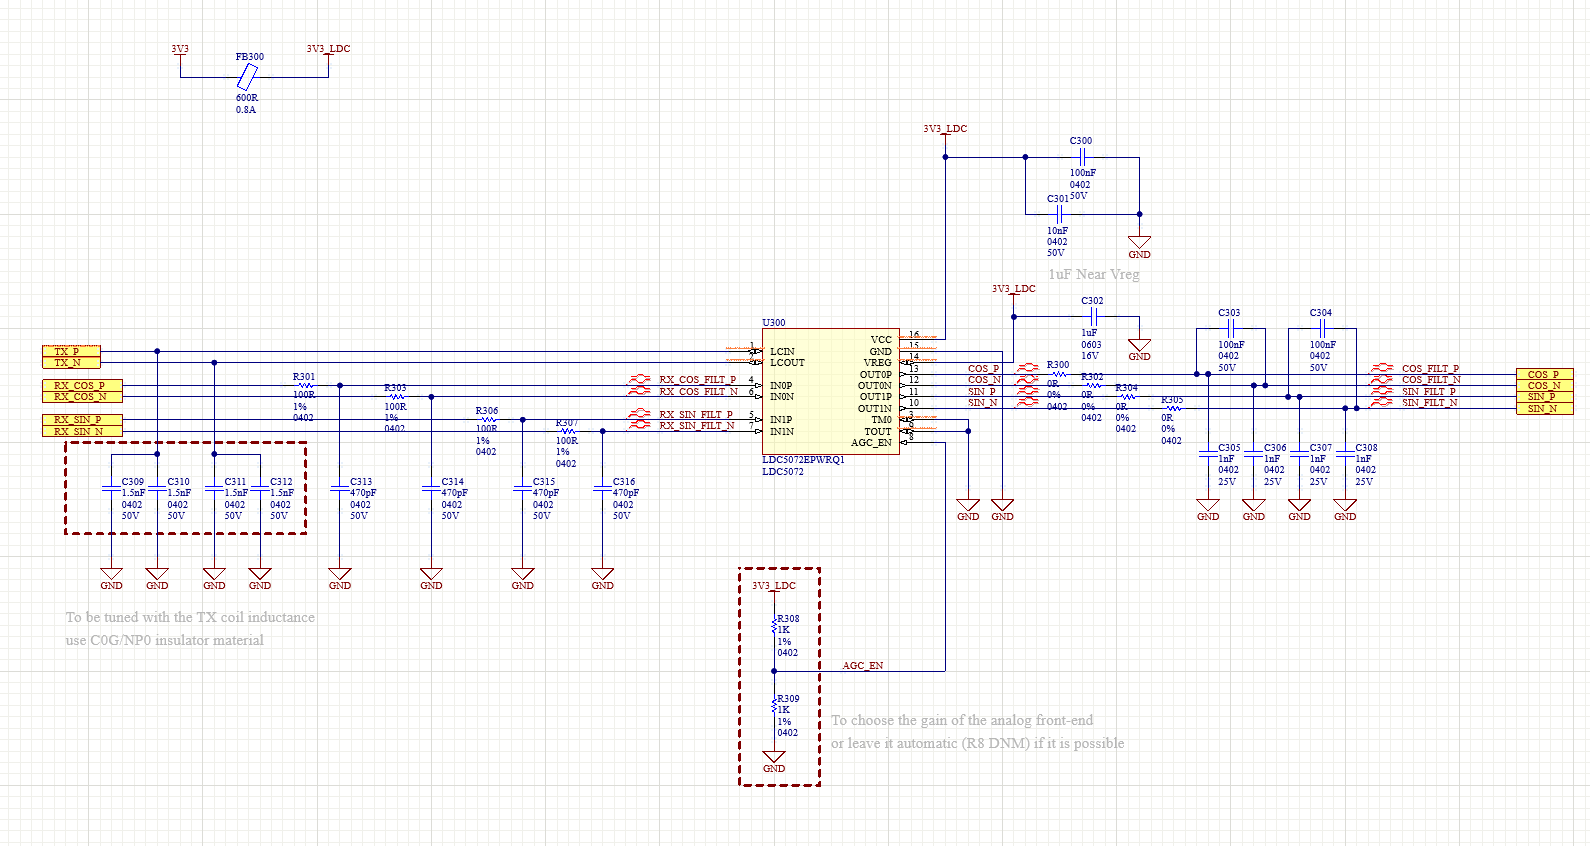
\includegraphics[width=\linewidth]{img/hw_block_coil_if_ic.png}
    \caption{Coil interface IC schematic}
    \label{HW_BLOCK_COIL_IF_IC}
\end{figure}

The outputs of the coil interface \ac{IC} are directly the demodulated sinewaves, that
can be directly connected to the microcontroller ADC input if their amplitude is 
high enough.

The next block is infact composed of the \ac{MCU} (figure \ref{HW_BLOCK_MCU}) which 
acquires the analog signals, processes them and produce the incremental encoder 
pulses.

\begin{figure}[h]
    \centering
    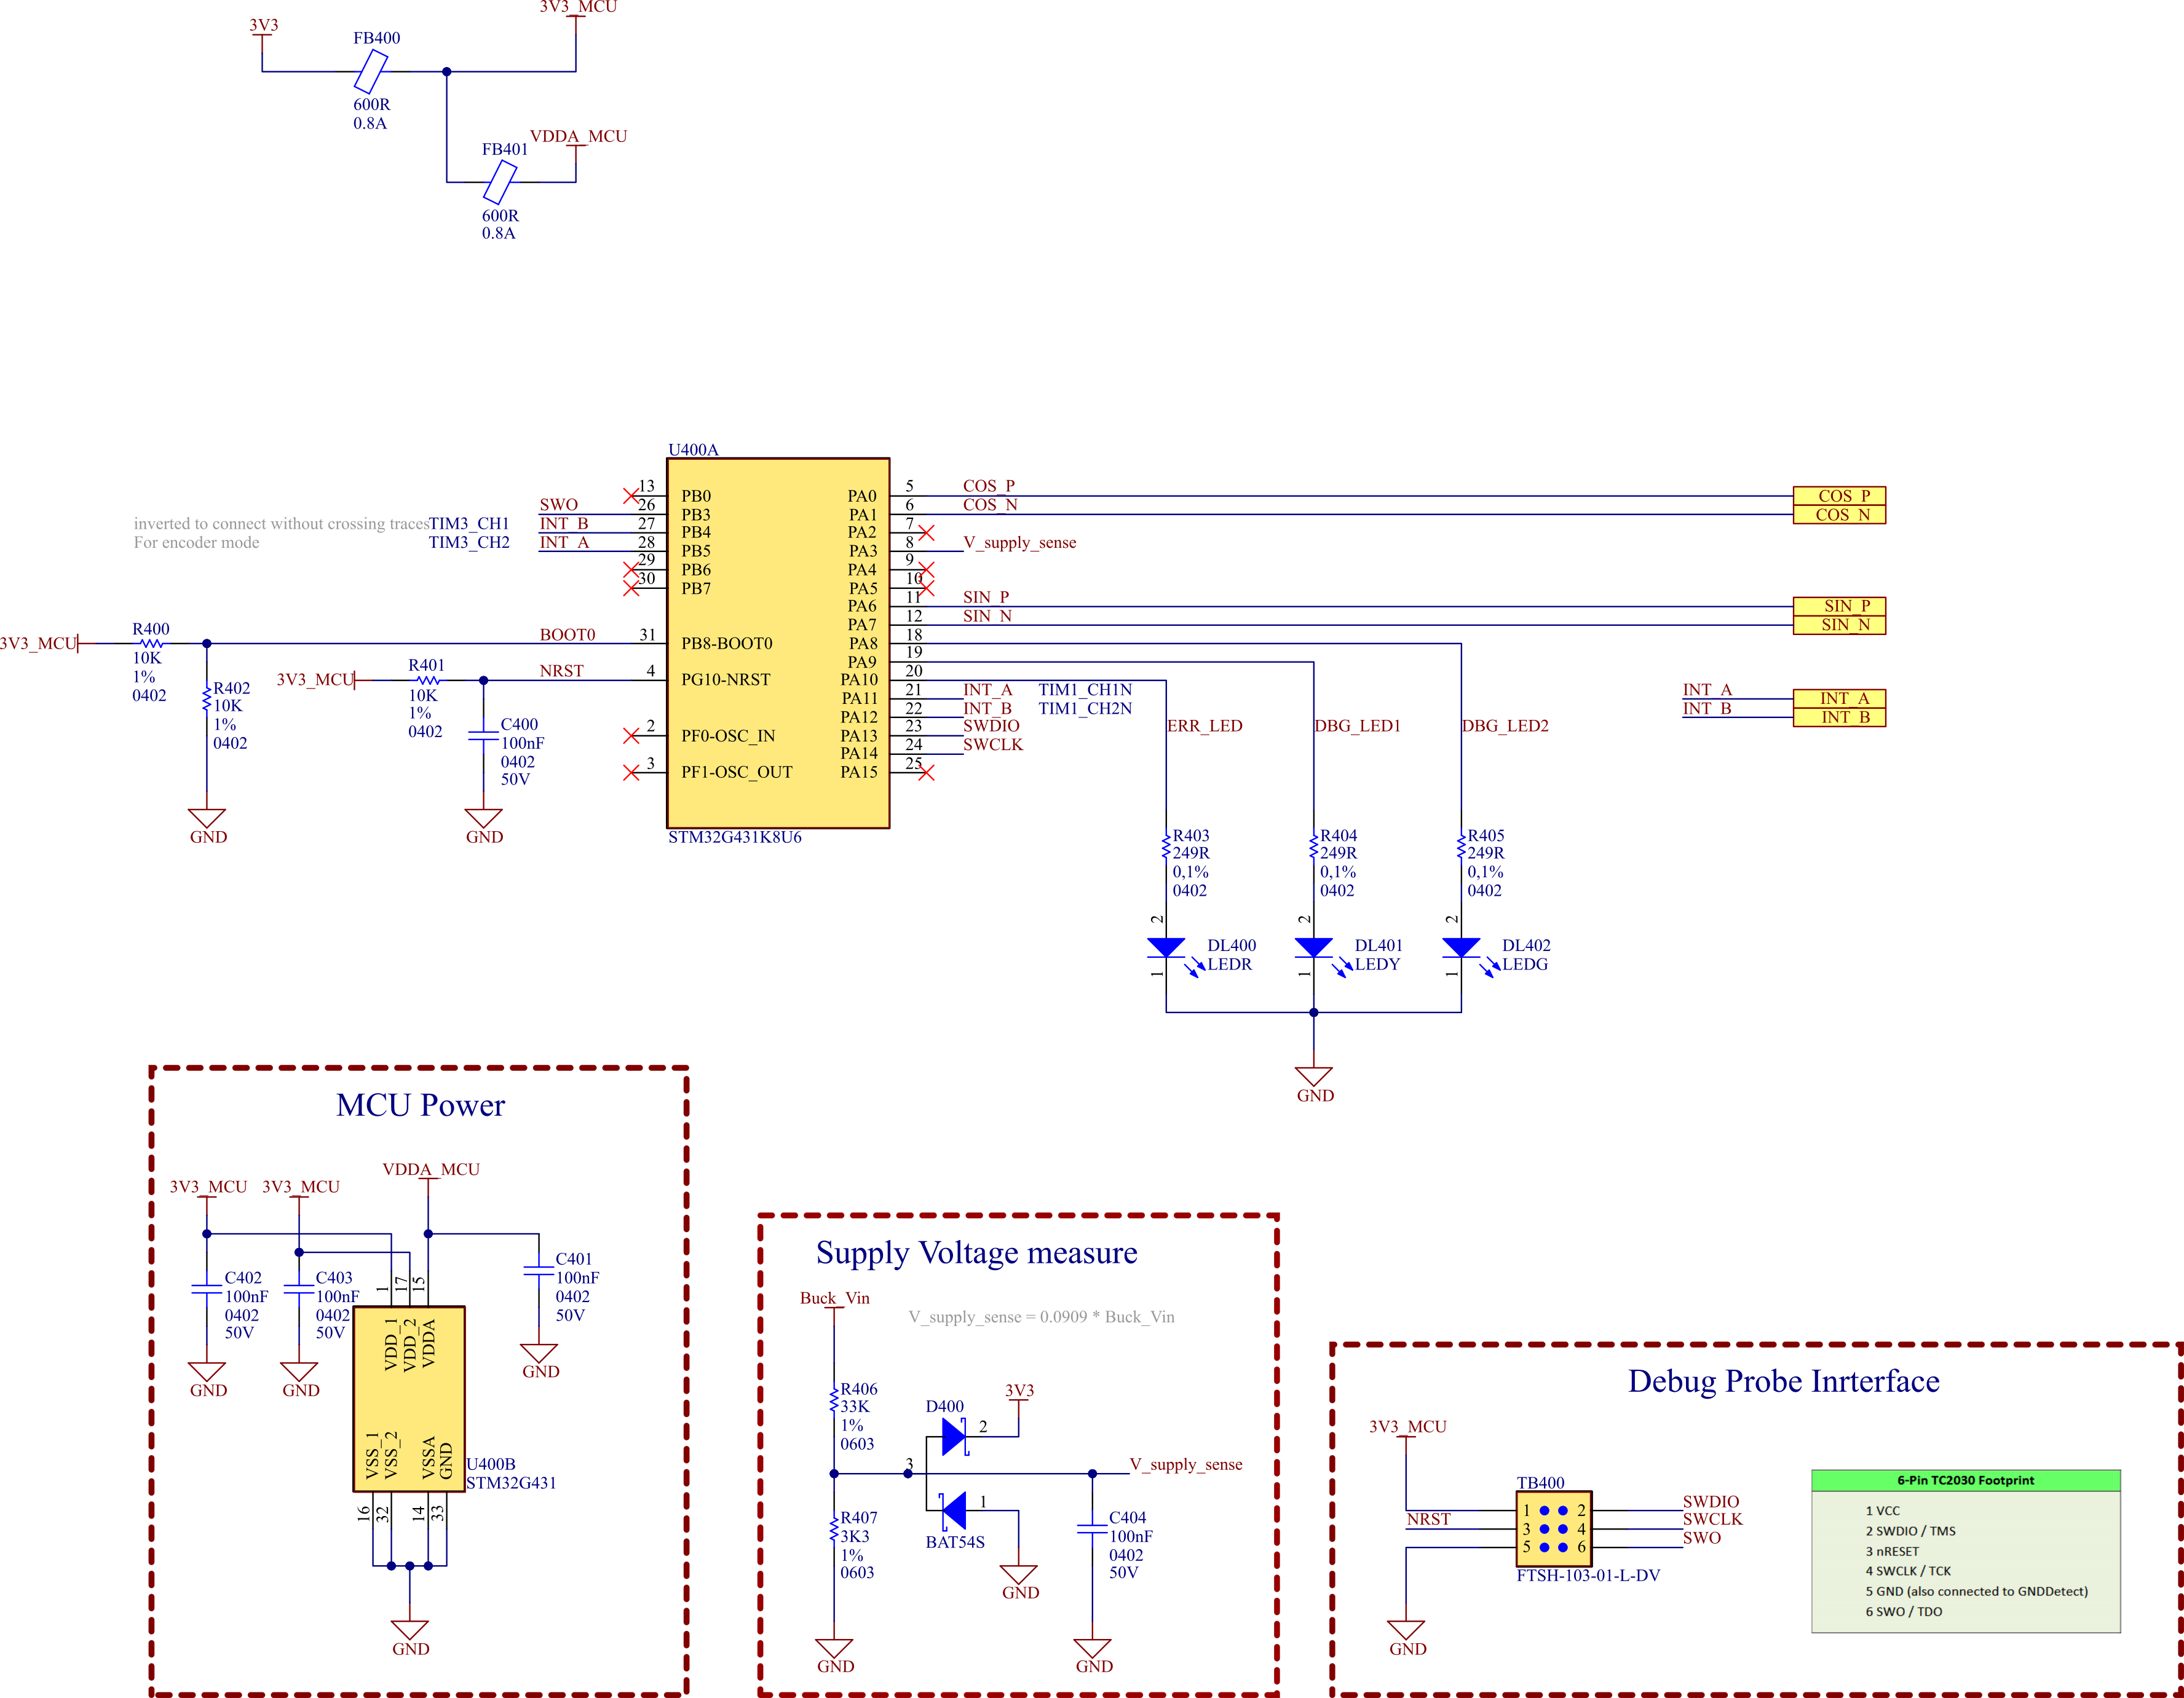
\includegraphics[width=\linewidth]{img/hw_block_mcu.png}
    \caption{MCU schematic}
    \label{HW_BLOCK_MCU}
\end{figure}

Finally these pulses are used to drive some open collector output transistors
to bring the signals on the sensor output pads (figure \ref{HW_BLOCK_OD}).

\begin{figure}[h]
    \centering
    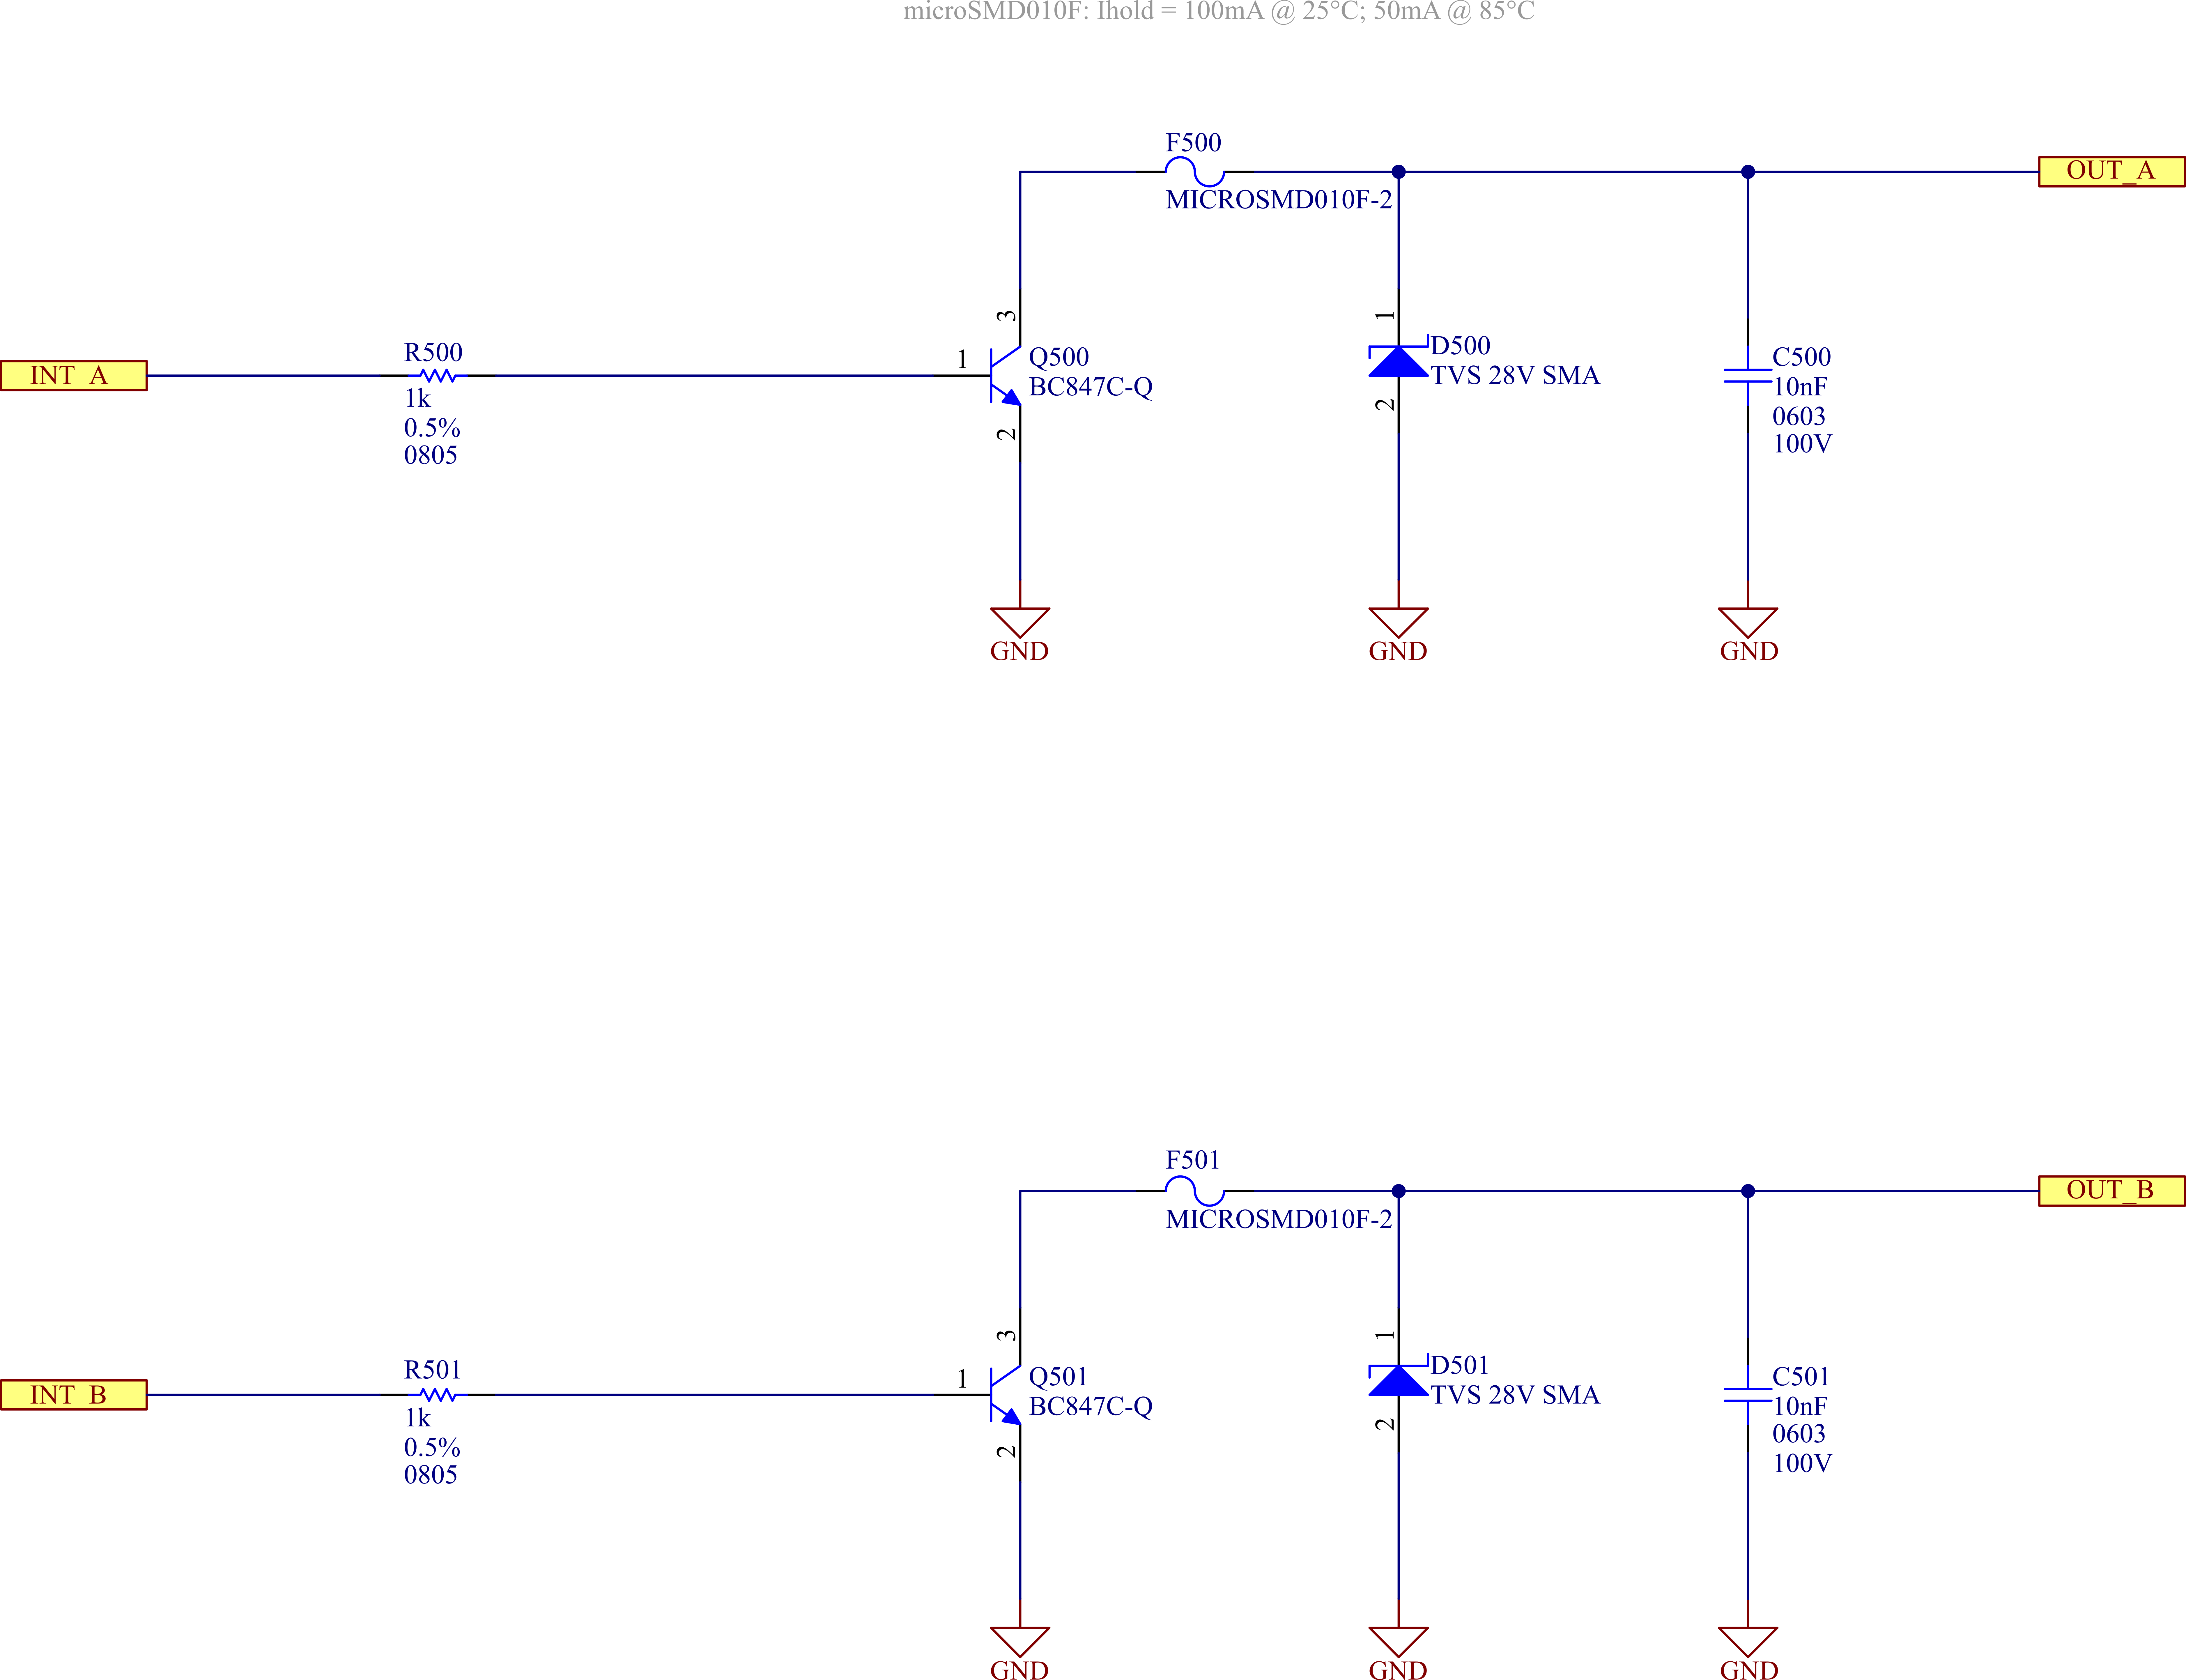
\includegraphics[width=\linewidth]{img/hw_block_od.png}
    \caption{Output drivers schematic}
    \label{HW_BLOCK_OD}
\end{figure}

\end{document}